% !TEX program = xelatex
\documentclass{article}
% \usepackage[utf8]{inputenc}
% \usepackage[T1]{fontenc}
% \usepackage[english]{babel}
% \usepackage{csquotes}

% with xelatex
% \usepackage{fontspec}  % fontspec et xunicode sont facultatifs
% \usepackage{xunicode}  % pour les versions postérieures à 2018.

\usepackage[a4paper, left=2.5cm,right=2.5cm,top=2.5cm,bottom=2.5cm]{geometry}
\setlength{\parindent}{1em}
% \setlength{\parskip}{1em}
\usepackage{indentfirst}

\usepackage[sfdefault,lining]{FiraSans} %% option 'sfdefault' activates Fira Sans as the default text font
\usepackage[fakebold]{firamath-otf}
\renewcommand*\oldstylenums[1]{{\firaoldstyle #1}}

\usepackage[none]{hyphenat}

\usepackage{graphicx}
\usepackage{float}
\usepackage{wrapfig}

\usepackage{enumitem}

\usepackage[language=australian, style=ieee]{biblatex}

\usepackage[hidelinks]{hyperref}

\title{
  
\includegraphics[width=0.4\textwidth]{../Images/Logo_Mines_ParisTech.png}\\
  \vspace{1em}
  \textbf{Monoclonal Antibody Therapy}
}
\author{Louis-Justin Tallot}
\date{February 2022}


\bibliography{../Bibliography/report_therapy_monoclonal_antibodies}

\begin{document}

  \maketitle

  \section*{Introduction}
  Monoclonal antibody therapy is a therapeutic strategy developed in the 1970s
that uses monoclonal antibodies to bind to specific targets such as viruses or tumor cells.
Indeed, monoclonal antibodies -- produced from a single white blood cell clone --
have high specificity to one epitope, and therefore can be used to specifically target
an antigen.

This paper will examine the scientific aspects of monoclonal antibody therapy,
such as the way they are produced and how they act when released as a drug.
The clinical and commercial aspects of this therapeutic way will also be examined.


  \section{What is a monoclonal antibody ?}

    \subsection{What is an antibody ?}
    First of all, let us examine what an antibody is, and see how this
type of molecules possesses remarkable properties that make it suitable
for therapeutic use.

An antibody (also known as Immunoglobulin) is a protein produced by the 
body's immune system that binds to a specific antigen. It is composed of four
polypeptide chains: two identical heavy chains 
and two identical light chains \cite{davies_antibody_1993}. 

The way this chains are self-assembled gives the protein a Y-shaped structure. 
Each of them possesses a terminal high-variability domain, which when grouped spatially
together forms a binding site that can be adapted to a wide variety of antigens.

\begin{figure}[!h]
    \begin{minipage}{0.495\textwidth}
        \centering
        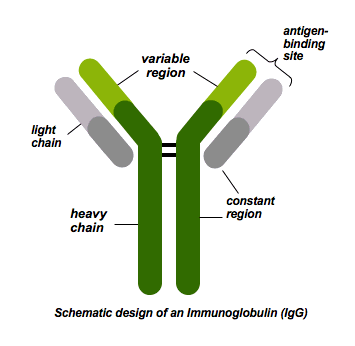
\includegraphics[width=\textwidth]{../Images/schematics_antibody.png}
        \caption{Schematic representation of an antibody} 
        \label{fig:schematics_antibody}
    \end{minipage}\hfill
    \begin{minipage}{0.495\textwidth}
        \centering
        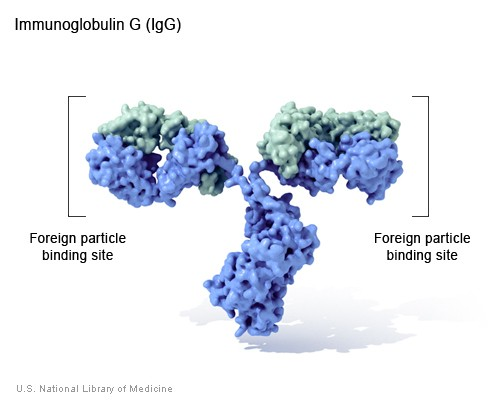
\includegraphics[width=\textwidth]{../Images/immunoglobulin_3D_model.jpg}   
        \caption{3D model of an antibody}
        \label{fig:immunoglobulin_3D_model}
    \end{minipage}
\end{figure}


The variation between immunoglobulins in the low-variability domain
creates multiple antibody classes, also known as \emph{isotypes} :
IgA, IgD, IgE, IgG, or IgM. They all have different functions, but act
following the same general principles that will be discussed later in this paper.


The most important one are :
\begin{itemize}
    \item IgG, which represents $75\%$ of serum antibodies
    in humans. It is involved in the immunity transmitted by a mother
    to her newborn, protecting the child for the first six months of life
    before it can acquire its own immune memory.
    \item IgM, which auto-assembles to form a pentamer, is the largest
    antibody and one of the first to response to an antigen intrusion.
\end{itemize}





    \subsection{Difference between monoclonal and polyclonal antibodies}
    \begin{frame}{Monoclonal \textit{versus} polyclonal antibodies}
    \begin{minipage}{0.5\textwidth}
        \begin{block}{Monoclonal antibody}

            \begin{itemize}
                \item Single antibody species
                \item Binds to a unique specific site
                \item Expensive to produce
            \end{itemize}
        \end{block}

        \begin{block}{Polyclonal antibody}
            \begin{itemize}
                \item Multiple antibody species
                \item Binds to multiple, less specific sites
                \item Cheap to produce
            \end{itemize}
        \end{block}
    \end{minipage}\hfill
    \begin{minipage}{0.45\textwidth}
        \begin{figure}
            \centering
        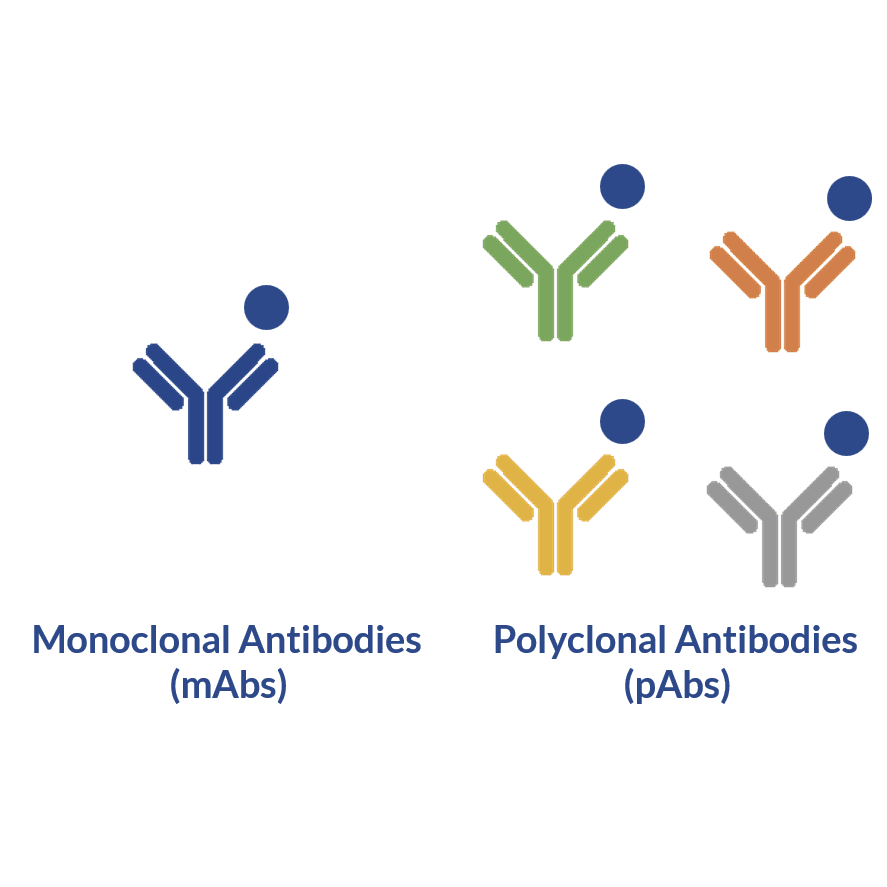
\includegraphics[width=\textwidth]{../Images/schematics_mono_poly.png}
        \caption{Comparison between monoclonal and polyclonal antibodies}
        \end{figure}    
    \end{minipage}
\end{frame}

    \subsection{Production of monoclonal antibodies}
    \label{sec:monoclonal_antibody_production}
    We will now examine the details of monoclonal antibody production.
It is done in multiple steps, as summarized on figure \ref{fig:Monoclonal_Antibody_Production}.

\begin{figure}[H]
    \begin{center}
        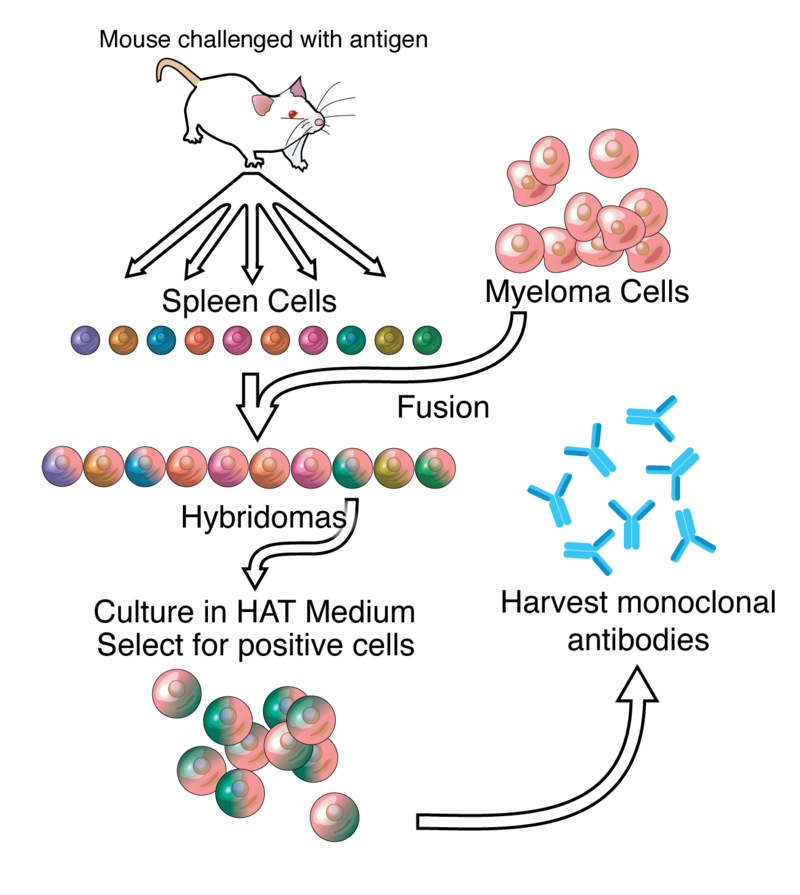
\includegraphics[width=0.4\textwidth]{../Images/mab_hybridomas.png}
        \caption{Monoclonal antibody production}
        \label{fig:Monoclonal_Antibody_Production}
    \end{center}
\end{figure}


\subsubsection{Step 1 : Immunization}

In order to begin the production of monoclonal antibodies, it is first
needed to immunize an animal with the antigen of interest. Typically, 
mice are used for this process \cite{leenaars_critical_2005}. 
An \emph{immunogen}, \textit{i.e} an antigen due to induce an immune response
in the animal, is then injected into the animal, along with an adjuvant
aiming at enhancing the immune response.


\subsubsection{Step 2 : Fusion and selection}

\subsubsection{Step 3 : Screening}

\subsubsection{Step 4 : Characterization}

\subsubsection{Step 5 : Production}

  \section{How are monoclonal antibodies used for therapy ?}
  In the first part of this paper, we have described monoclonal
antibodies, seen their advantages and how they
can be industrially produced. In this second part, we are going
to see the different mechanisms by which antibodies can react to 
a pathogen infection, and then how these abilities can be put
into action to create drugs.

    \subsection{Mechanisms of action of a monoclonal antibody}
    First of all, let us examine the different ways by which
antibodies are naturally used by the immune system to combat
a pathogen infection. There are four of them, complementary of each other.

The key point here is that the antibodies allow for a specific recognition
of an antigen, and allow the immune system to act on it after it has
been detected. The antibodies on their own do not kill nor suppress any pathogen,
but act as the "recognition" part of the whole immune system.

\subsubsection{Antigen neutralization}

\begin{figure}[H]
    \begin{minipage}{0.55\textwidth}
        The most simple way antibodies can act against a pathogen is by
        \emph{neutralization} : the antibodies specific to an epitope of the
        antigen bind to this epitope and form together a complex that surround
        the pathogen \cite{langermans_antimicrobial_1994}.
        It is thus geometrically prevented to act as it normally would 
        by infecting the nearby cells.

        Antibodies acting in this manner are called \emph{neutralizing antibodies}
        or NAbs. The neutralized pathogen cannot approach the cell and
        bind to its surface receptors, thus making it ineffective. 
        The resulting complex can then be eliminated.
    \end{minipage}\hfill
    \begin{minipage}{0.35\textwidth}
        \centering
        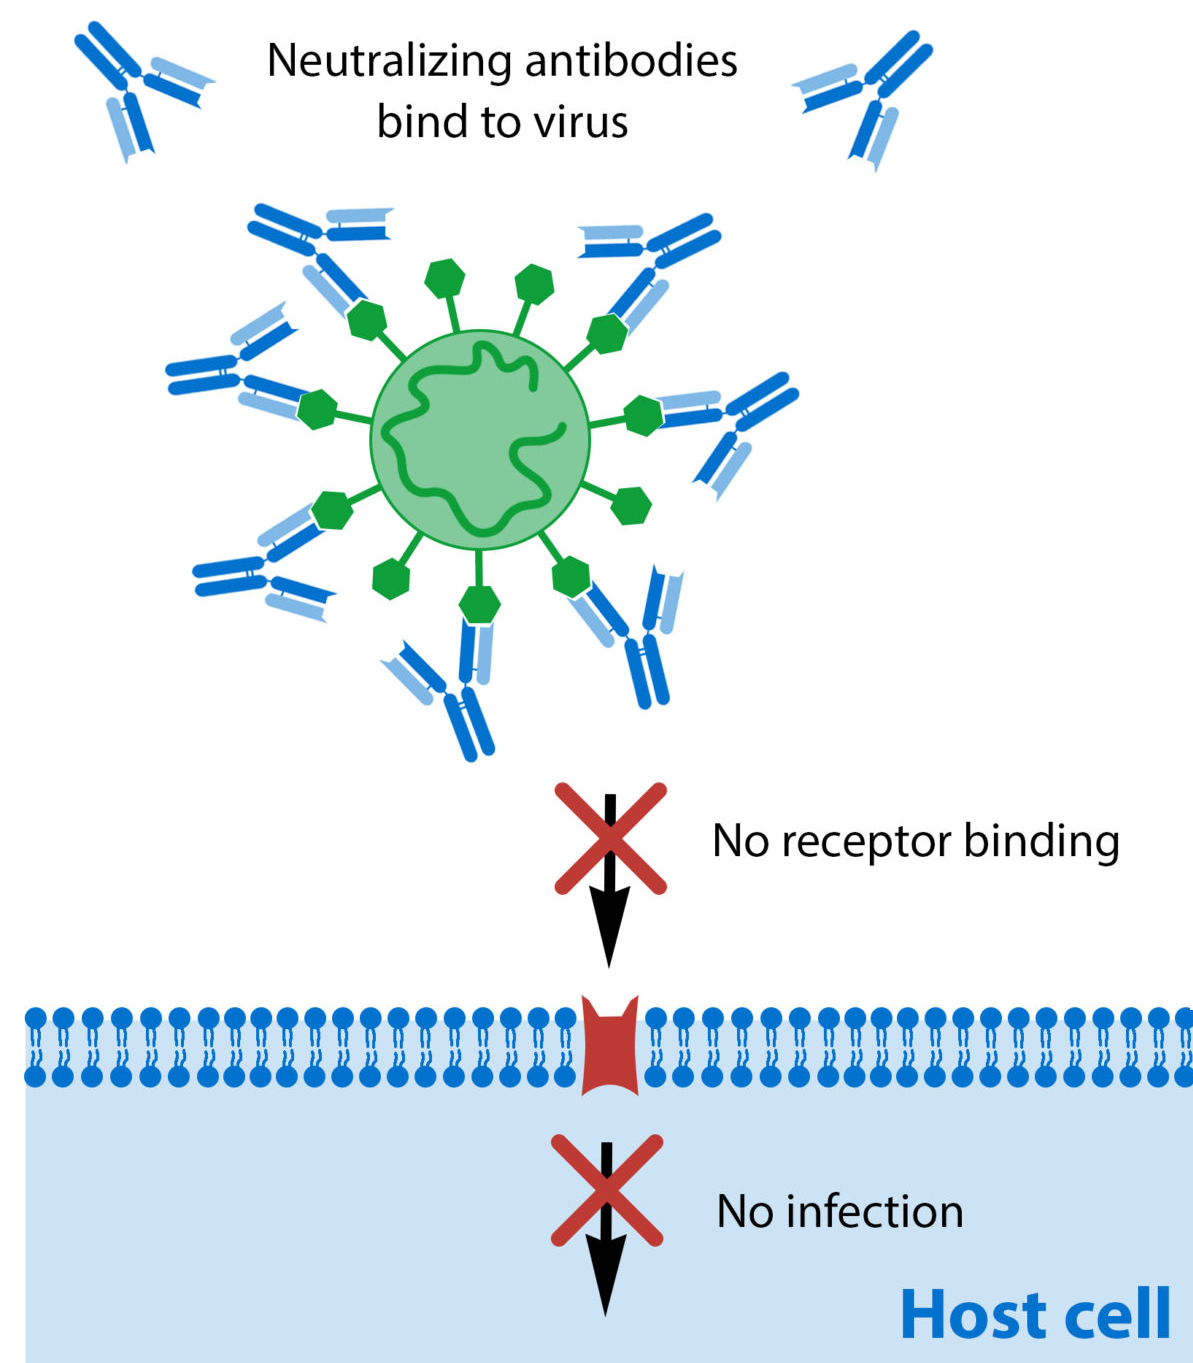
\includegraphics[width=\textwidth]{../Images/neutralization.png}   
        \caption{Neutralization of a pathogen by antibodies}
        \label{fig:neutralization}
    \end{minipage}
\end{figure}


\subsubsection{Antibody-Dependent Cellular Phagocytosis (ADCP)}

Another way by which antibodies help acting against a pathogen is very
close to neutralization. Indeed, once an antigen-antibody complex has been
created, some Fc receptor expressive immune effector cells can come into action
and act on the pathogen. 

\begin{figure}[H]
    \begin{minipage}{0.49\textwidth}
        \centering
        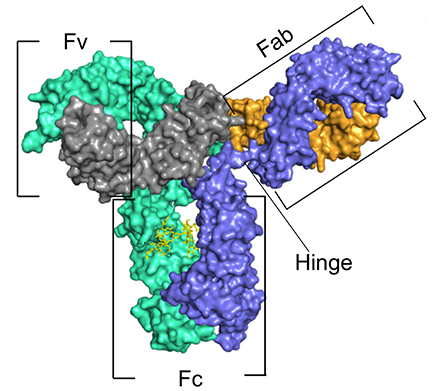
\includegraphics[width=0.9\textwidth]{../Images/antibody_domains.png}   
        \caption{The different domains of an immunoglobulin}
        \label{fig:antibody_domains}
    \end{minipage}\hfill
    \begin{minipage}{0.49\textwidth}
        \centering
        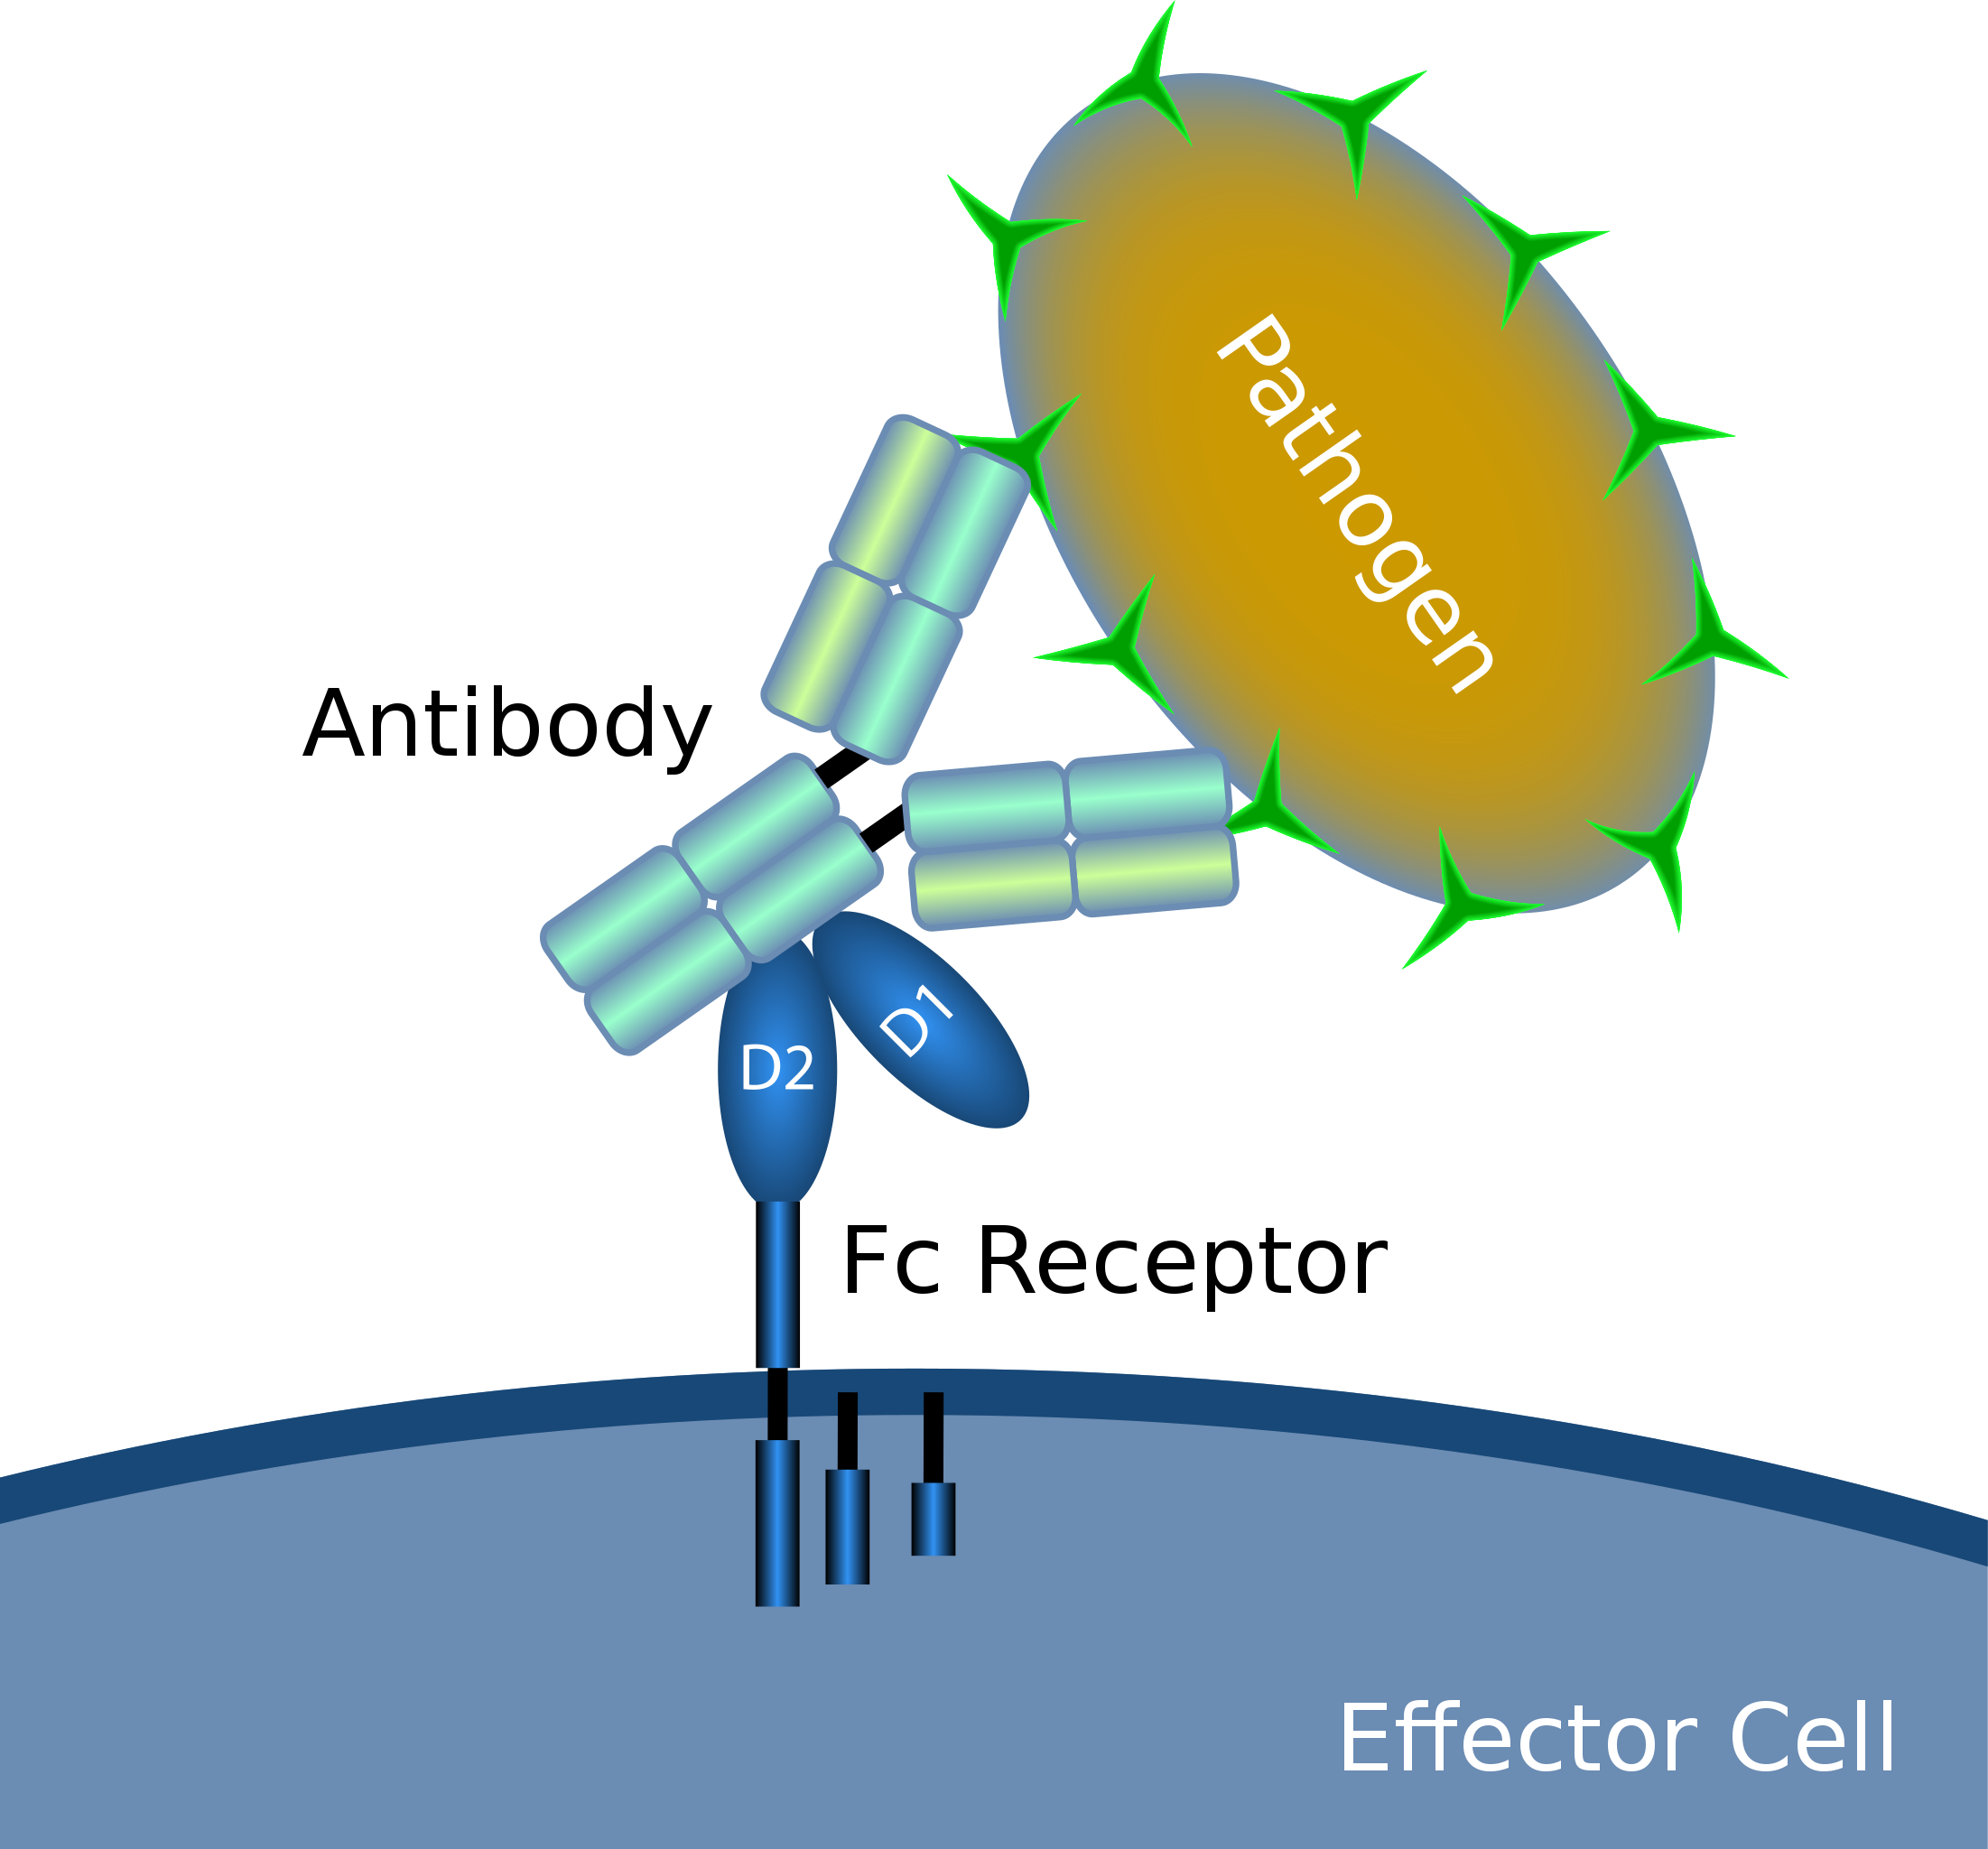
\includegraphics[width=0.9\textwidth]{../Images/Fc_receptor_interaction.png}   
        \caption{Interaction between the Fc receptor of an effector cell 
        and the Fc domain of an antibody attached to a pathogen}
        \label{fig:Fc_receptor_interaction}
    \end{minipage}
\end{figure}

Some cells, such as \emph{macrophages}, \emph{natural killer cells} or B lymphocytes, 
can bind to the Fc domain (shown on figure \ref{fig:antibody_domains})
of immunoglobulins attached to pathogens or infected -- or tumor -- cells
using their Fc receptors -- which are trans membrane proteins \cite{fridman_fc_1991}, 
as shown on figure \ref{fig:Fc_receptor_interaction}. 
The phagocytic or cytotoxic activity of the cell is then activated \cite{tay_antibody-dependent_2019}.
This mechanism allow for the precise elimination of antigenic material, the antibodies
permitting specific detection of the pathogen or undesirable cell, and the effector cells
killing and eliminating the antigen.

\begin{figure}[H]
    \begin{minipage}{0.49\textwidth}
        \centering
        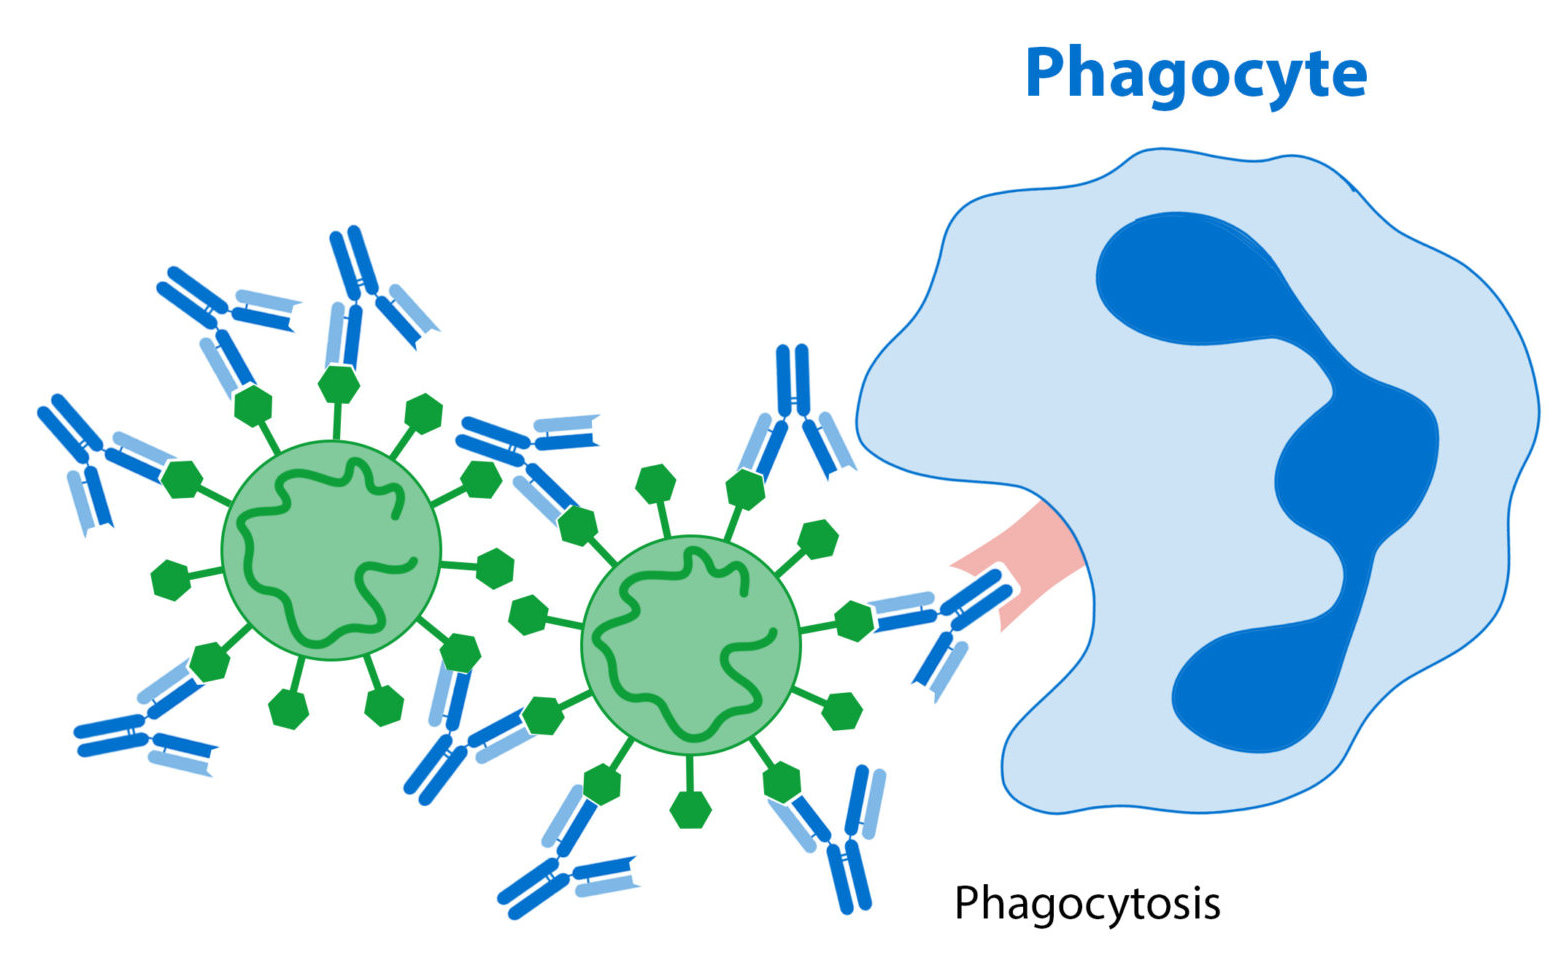
\includegraphics[width=0.9\textwidth]{../Images/phagocytosis.png}   
        \caption{Phagocytosis of a pathogen detected by antibodies}
        \label{fig:phagocytosis}
    \end{minipage}\hfill
    \begin{minipage}{0.49\textwidth}
        \centering
        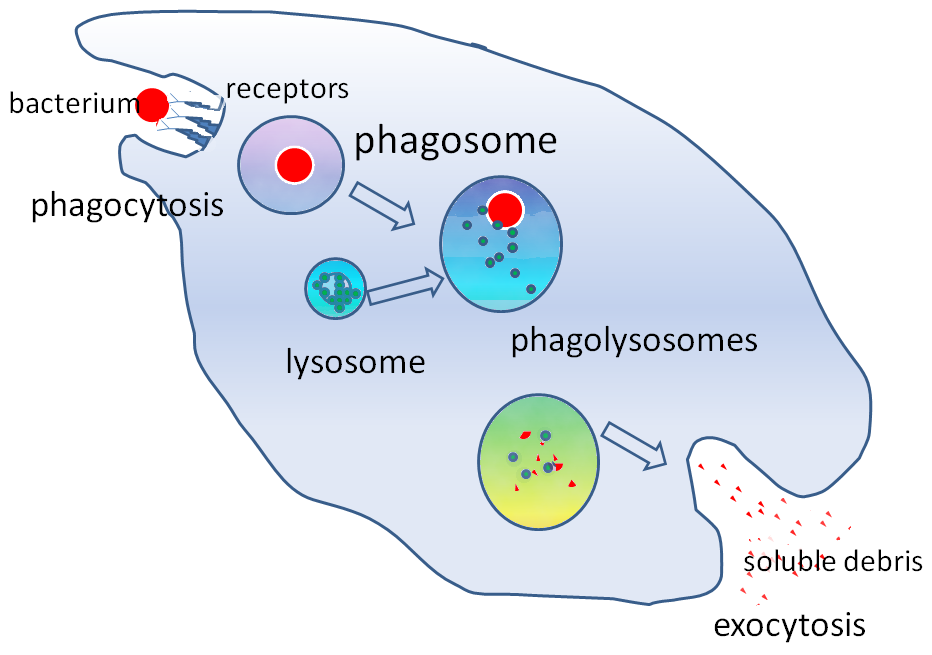
\includegraphics[width=0.9\textwidth]{../Images/phagocytosis_steps.png}   
        \caption{The steps of phagocytosis}
        \label{fig:phagocytosis_steps}
    \end{minipage}
\end{figure}

To speak more specifically about phagocytosis, this mechanism is of high importance
in a multicellular organism immune system ; it allows removal of large particles
(bigger than $0.5$ µm) such as dead cells, bacteria, mineral particles.

Phagocytosis occurs in multiple phases \cite{uribe-querol_phagocytosis_2020}
as seen on figure \ref{fig:phagocytosis_steps} : 
\begin{itemize}
    \item Detection of the particle that is going to be ingested
    \item Internalization and formation of a vacuole called \emph{phagosome}
    \item Maturation of the phagosome which is transformed in a \emph{phagolysosome}.
\end{itemize}

Degradation of the cell, bacteria or virus ingested is performed in the phagolysosome.
Indeed, the conditions inside the vacuole are extreme : the Ph is extremely acidic,
around $4,5$ due to the presence of many Vacuole ATPases \cite{uribe-querol_phagocytosis_2020},
the high concentration in $\text{H}^+$ ions being compensated for
by $\text{Cl}^-$ anions \cite{gordon_phagocytosis_2016}. 
Moreover, the phagolysosome membrane possesses the NADPH oxidase complex 
which produces Reactive Oxygen Species (ROS) like $\text{O}^{2-}$, which can then
dismutate to $\text{H}_2\text{O}_2$, which can itself react with $\text{Cl}^-$ ions
to form hypochlorous acid which is a highly active microbicidal substance while
being non-toxic to biological tissues \cite{eryilmaz_antimicrobial_2013}.
These conditions allow for the destruction of the cytoskeleton and the 
recycling of the components of the ingested cell.


It should be noted that although all types of cells can perform phagocytosis,
only professional cells such as macrophages, monocytes or dendritic cells can
do so with high efficiency. Finally, phagocytosis does not only act as an
immune response to an infection by a pathogen, but is a normal part of the
life cycle of tissues, as dead tissues cell are recycled 
in this way \cite{arandjelovic_phagocytosis_2015}.

\subsubsection{Antibody-Dependent Cell Cytotoxicity (ADCC)}

\begin{figure}[H]
    \begin{minipage}{0.69\textwidth}
        \centering
        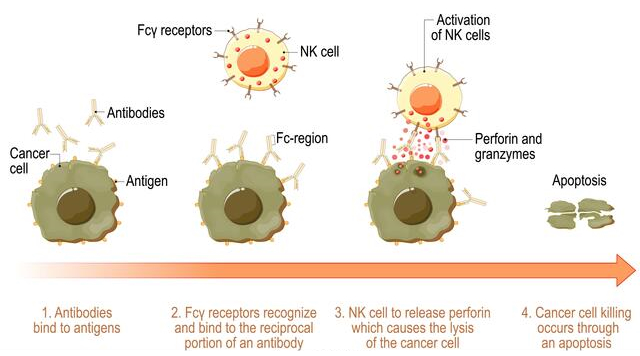
\includegraphics[width=0.7\textwidth]{../Images/ADCC.jpg}
        \caption{Mechanism of Antibody-Dependent Cell Cytotoxicity}
        \label{fig:ADCC}
    \end{minipage}\hfill
    \begin{minipage}{0.39\textwidth}
        \centering
        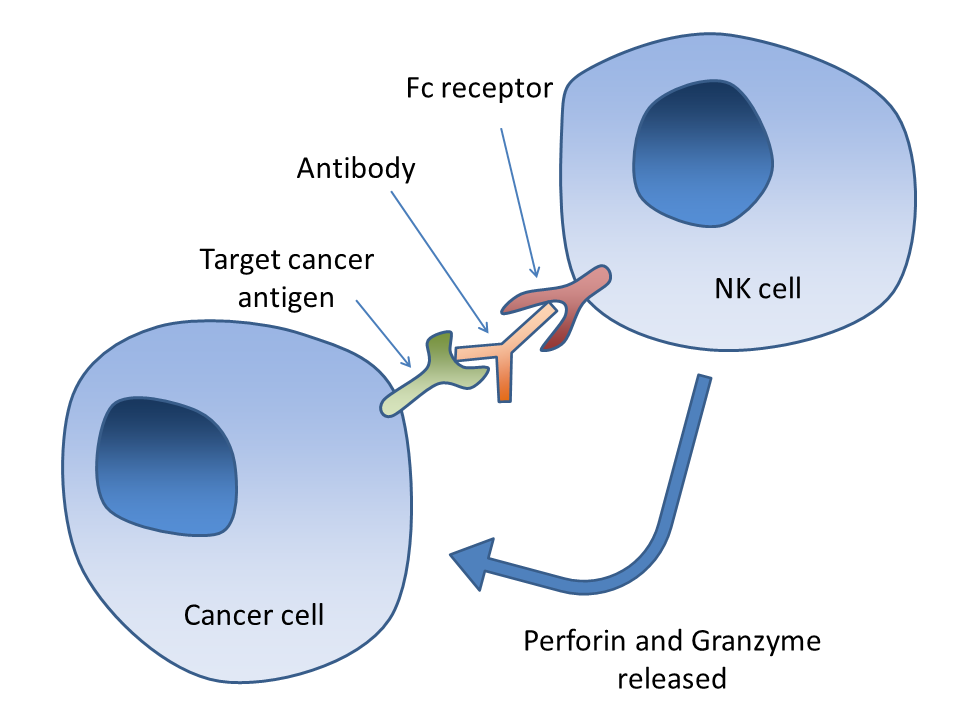
\includegraphics[width=0.9\textwidth]{../Images/Antibody-dependent_cell-mediated_cytotoxicity.png}   
        \caption{Action of a NK cell against a target cell}
        \label{fig:ADCC-NKcell}
    \end{minipage}
\end{figure}

Another way by which cytotoxicity is activated is called 
\emph{antibody-dependent cell cytotoxicity} (ADCC). In this process,
antibodies having recognized a pathogen will recruit a 
\emph{natural killer} cell (NK cell) using the cell's Fc receptors
like previously described.

This activates the NK cell action : it will release enzymes of which perforins
and granzymes. Perforins will create pores in the target cell's membrane and 
facilitate the entry of granzymes, which will induce the apoptosis
of the target cell \cite{paul_molecular_2017}.

\subsubsection{Complement-Dependent Cell Cytotoxicity (CDCC)}


    \subsection{Commercial uses}
    \begin{frame}{Commercial examples of the use of mAb}
    \begin{block}{Trastuzumab against HER2-positive breast cancer}
        \vspace{1em}
        \begin{minipage}{0.495\textwidth}
            \begin{figure}
                \centering
                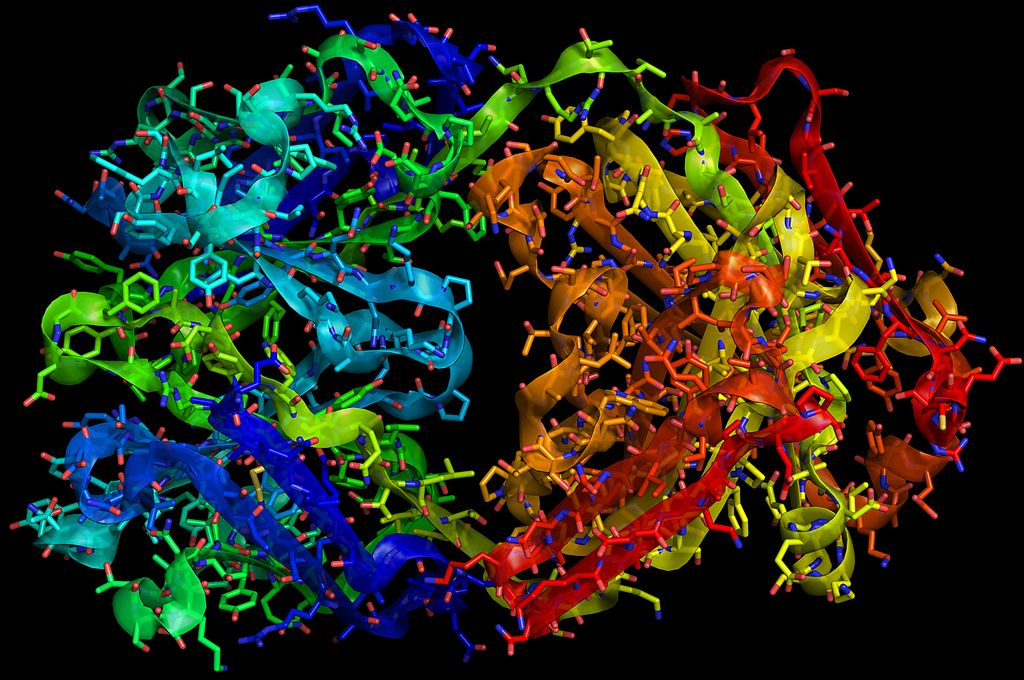
\includegraphics[width=\textwidth]{../Images/herceptin.jpg}
            \end{figure}  
        \end{minipage}\hfill
        \begin{minipage}{0.495\textwidth}
            \begin{figure}
                \centering
                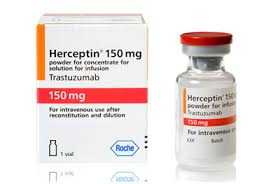
\includegraphics[width=\textwidth]{../Images/trastuzumab.jpg}
            \end{figure}    
        \end{minipage}
    \end{block}
\end{frame}

\begin{frame}{Commercial examples of the use of mAb}
    \begin{block}{Trastuzumab against HER2-positive breast cancer}
        % \vspace{1em}
        
        \begin{exampleblock}{Action mechanism}
            \begin{itemize}
                \item In the cancer cells, the HER2 protein is over-expressed
                \item The HER2 protein is a transmembrane protein, which then
                        proliferates along with the cancer cells
                \item Trastuzumab blocks HER2 activation and dimerization 
                \item The mAb also induces ADCC (Antibody Dependent Cell Cytotoxicity)
            \end{itemize}
        \end{exampleblock}

        \begin{exampleblock}{Treatment characteristics}
            \begin{itemize}
                \item 1-year long chemotherapy
                \item One injection every 3 weeks ($6$ mg/kg dose)
                \item Cost per patient : $17000$ €
            \end{itemize}
        \end{exampleblock}
    \end{block}

\end{frame}

\begin{frame}{Commercial examples of the use of mAb}
    \begin{block}{Trastuzumab against HER2-positive breast cancer}
        \begin{figure}
            \centering
            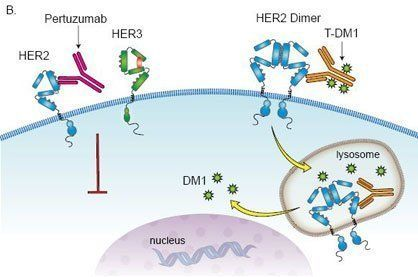
\includegraphics[width=0.8\textwidth]{../Images/her2_pertuzumab.jpg}
            \caption{HER2 dimerization and treatment by trastuzumab}
        \end{figure}
    \end{block}
\end{frame}


\begin{frame}{Commercial examples of the use of mAb}
    \begin{block}{Rituximab against lymphoma and leukemia}
        \vspace{1em}
        \begin{minipage}{0.495\textwidth}
            \begin{figure}
                \centering
                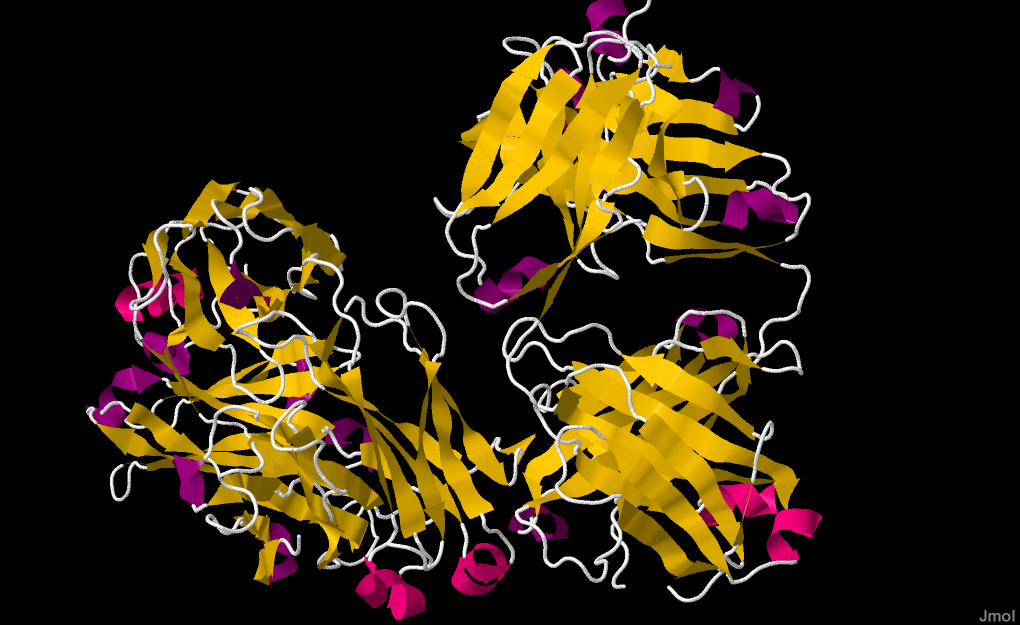
\includegraphics[width=\textwidth]{../Images/Rituximab.png}
            \end{figure}  
        \end{minipage}\hfill
        \begin{minipage}{0.495\textwidth}
            \begin{figure}
                \centering
                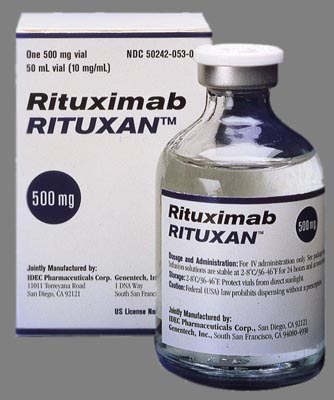
\includegraphics[width=0.8\textwidth]{../Images/rituxan.jpg}
            \end{figure}    
        \end{minipage}
    \end{block}
\end{frame}

\begin{frame}{Commercial examples of the use of mAb}
    \begin{block}{Rituximab against lymphoma and leukemia}
        \begin{exampleblock}{Action mechanism}
            \begin{itemize}
                \item In a lymphoma, 
            \end{itemize}
        \end{exampleblock}
        
        \begin{exampleblock}{Treatment characteristics}
            \begin{itemize}
                \item 1-year long chemotherapy
                \item One injection every 3 weeks ($6$ mg/kg dose)
                \item Cost per patient : $17000$ €
            \end{itemize}
        \end{exampleblock}
    \end{block}
\end{frame}



    \subsection{Market analysis}
    
  
  \section*{Conclusion}
  In conclusion, monoclonal antibodies are a promising therapeutic agent for
treatment of cancers and infectious diseases. They are very potent at neutralizing
a specific target and can then be used to eliminate it, either by leveraging the patient's
own immune system capabilities or by bringing a chemical agent attached to the antibody.

The therapeutic market for monoclonal antibodies is growing rapidly, valued
at $160$ billion dollars in 2020 and expected to grow threefold by 2030
\cite{terdale_monoclonal_2021} \cite{insights_monoclonal_2021}.
This growth is accompanied by an important research effort, the research market
being valued at $5,9$ billion dollars in 2020 and expected to grow
at an annual rate of $6 \%$ until 2028 \cite{markets_global_2021}.

Finally, around $500$ monoclonal antibodies have been discovered, leading To
the approval of nearly $100$ mAbs-based drugs. This presents a challenge for
researchers, fighting against viruses and cancers, but more importantly is a great
hope for humankind which can fight its most lethal diseases, even if it does so
at a high cost, and thus that only the richest countries can access such treatments.

% \appendix

  \printbibliography

  \listoffigures
\end{document}
